	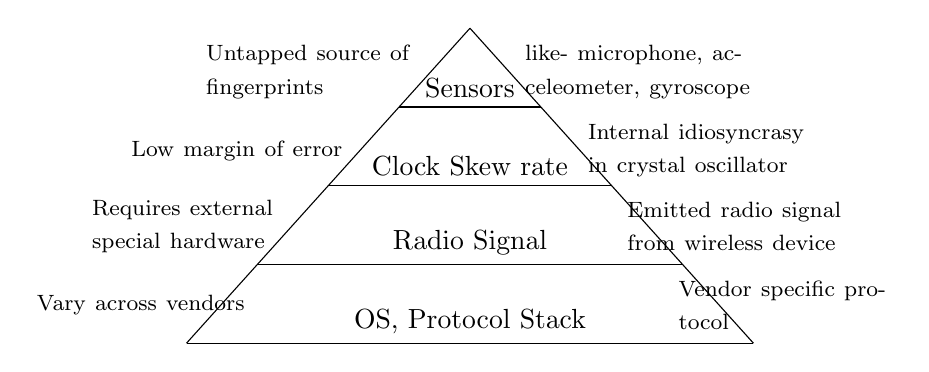
\begin{tikzpicture}[scale=1]

		\def \h {4};
		\def \f {0.9};

		\foreach \y in  {0,1,2,3} {
		    \def \w { \h*\f-\y*\f };
		    \def \v { \y*\f-\h*\f };
		    \draw (\v,\y) -- (\w,\y);
		}

		\draw (-\h*\f,0)  -- (0,\h);
		\draw (\h*\f,0)  -- (0,\h);
		\node (os) at (0,0) [above] {OS, Protocol Stack};
		\node (rf) at (0,1) [above] {Radio Signal};
		\node (cs) at (0,2) [above] {Clock Skew rate};
		\node (se) at (0,3) [above] {Sensors};


		\node [left of=os, xshift=-3cm, yshift=0.2cm, text width=3cm] {\footnotesize{Vary across vendors}};
		\node [left of=rf, xshift=-2.4cm, yshift=0.2cm, text width=2.8cm] {\footnotesize{Requires external special hardware}};
		\node [left of=cs, xshift=-1.8cm, yshift=0.2cm, text width=3cm] {\footnotesize{Low margin of error}};
		\node [left of=se, xshift=-1cm, yshift=0.2cm, text width=2.7cm] {\footnotesize{Untapped source of fingerprints}};

		\node [right of=os, xshift=3cm, yshift=0.2cm, text width=2.7cm] {\footnotesize{Vendor specific protocol}};
		\node [right of=rf, xshift=2.5cm, yshift=0.2cm, text width=3cm] {\footnotesize{Emitted radio signal from wireless device}};
		\node [right of=cs, xshift=2cm, yshift=0.2cm, text width=3cm] {\footnotesize{Internal idiosyncrasy in crystal oscillator}};
		\node [right of=se, xshift=1.2cm, yshift=0.2cm, text width=3cm] {\footnotesize{like- microphone, acceleometer, gyroscope}};
	\end{tikzpicture}